\documentclass[tikz,border=6pt]{standalone}
\usepackage{times}
\usepackage{pgfplots}
\pgfplotsset{compat=1.18}
\begin{document}
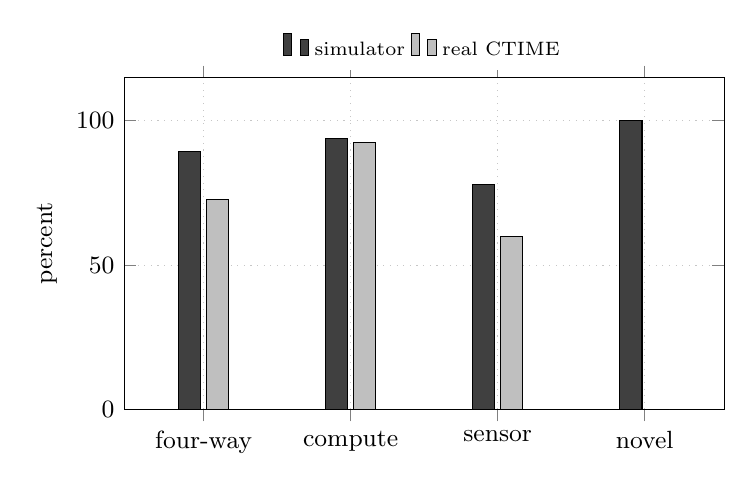
\begin{tikzpicture}
\begin{axis}[
  ybar,
  bar width=8pt,
  width=9.2cm,
  height=5.8cm,
  ylabel={percent},
  ymin=0, ymax=115,
  enlarge x limits=0.18,
  symbolic x coords={four-way,compute,sensor,novel},
  xtick=data,
  legend style={at={(0.5,1.02)}, anchor=south, legend columns=2, font=\scriptsize, draw=none},
  grid=major,
  major grid style={dotted, gray!45},
  tick label style={font=\small},
  label style={font=\small},
]
\addplot[fill=black!75] coordinates {(four-way,89.3) (compute,93.9) (sensor,77.8) (novel,100.0)};
\addlegendentry{simulator}
\addplot[fill=black!25] coordinates {(four-way,72.8) (compute,92.5) (sensor,60.0) (novel,0.0)};
\addlegendentry{real CTIME}
\end{axis}
\end{tikzpicture}
\end{document}
